\documentclass[../main.tex]{subfiles}

\begin{document}
    \chapter{Approach}

    \section{Grad-CAM}
    Gradient-weighted Class Activation Mapping~\cite{gradcam}. Technique for producing visual explanations
    about why a Convolutional Neural Network opted for a certain class. The technique is applicable to a wide
    variety of tasks, ranging from image captioning to visual question answering to reinforcement learning, and
    also to a wide variety of CNN architectures. In the context of this work, we'll use this technique to
    produce visuals for an object classification task.
    This technique was designed as a visualization tool to better understand how CNNs reason and to improve
    their interpretability, which is a fundamental property to have for AI systems that wants to be deployed
    in the real world.
    We extracted the Grad-CAM visualization from the last convolutional layer because, as also the authors
    or the technique note, the last convolutional layer is the best compromise between high-level semantics and spatial
    localization. The former is a general property of deep learning models: the further the layer from the input,
    the more high-level and meaningful features one can expect to be extracted. The latter is a property of
    Convolutional Feature Maps, which are designed to retain as much spatial information as possible about
    the data.
    The high-level architecture of the method can be seen in the following figure.

	\begin{figure}[h!]
    	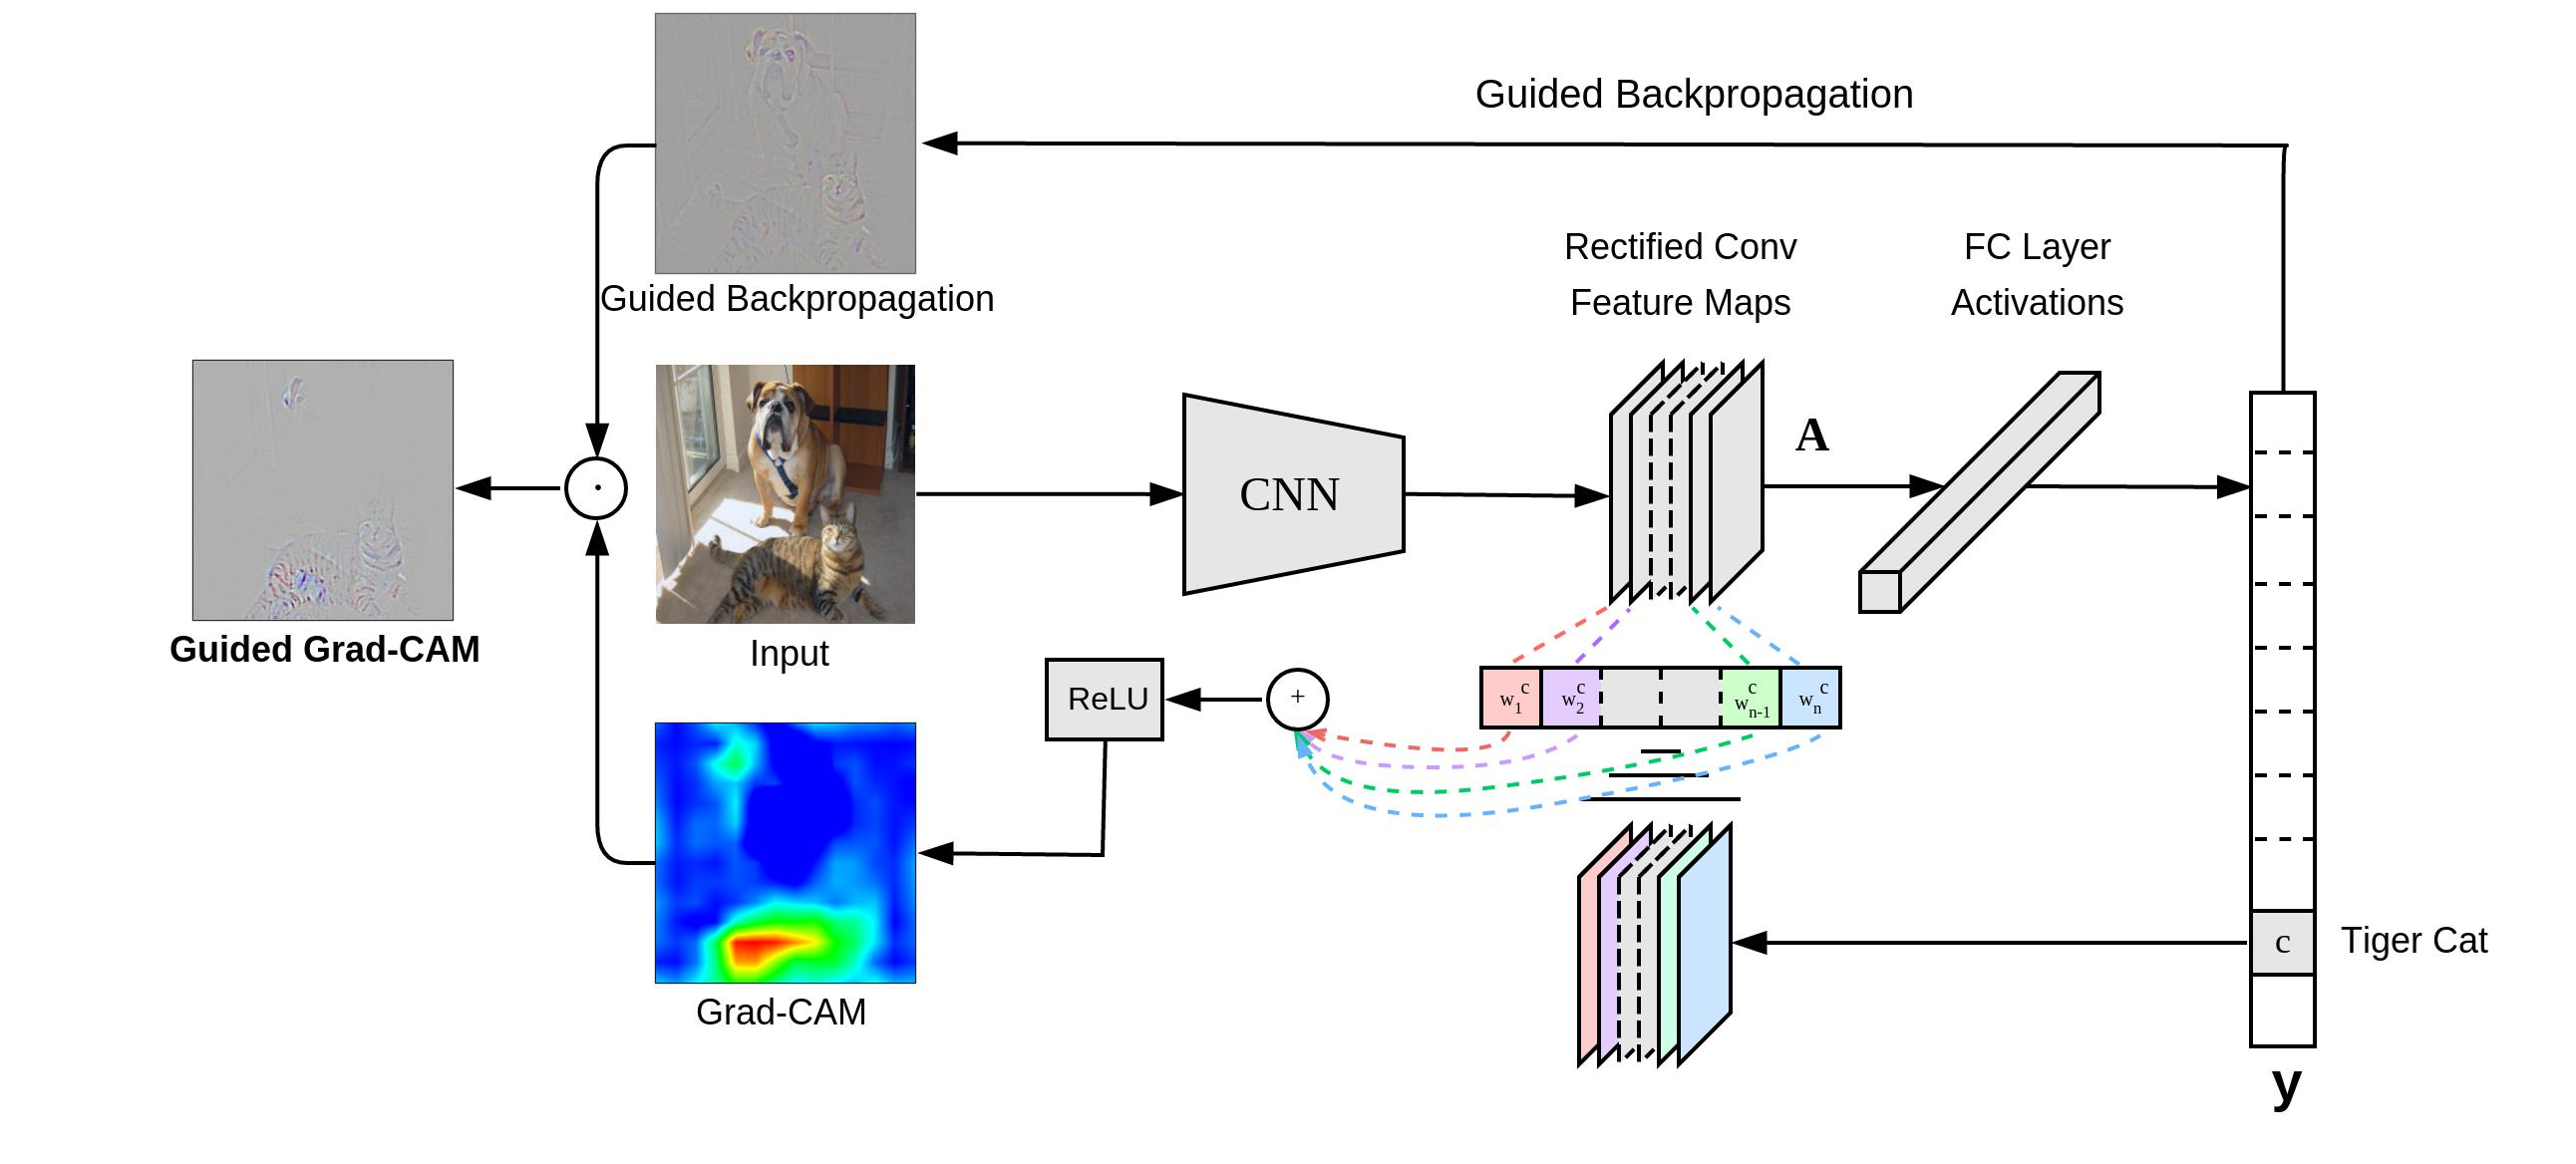
\includegraphics[width=\linewidth]{img/gradcam-architecture.png}
	    \caption{Grad-CAM Architecture, taken from~\cite{gradcam}}\label{fig:gradcam-architecture}
	\end{figure}

    Basically, the input image is forward propagated through the network in order to compute the softmax scores
    of the last layer, which we call $y^{c} = f(x)$, where $f()$ is the input-output network mapping.
    If we were training the network, at this point we would have computed the gradients of the
    last layer neurons with respect to some loss function, like cross-entropy. Instead, in Grad-CAM, we manually
    create these gradients. In particular, we set them to one for the neuron corresponding to the class of interest,
    while all the other neurons are set to zero.
    $$ \frac{\partial y^{c}}{\partial \theta_{output}} = [0, 0, \ldots 1, 0, 0, \ldots] $$
    Then, we backward propagate these gradients through the network untill
    the last convolutional layer, where the Grad-CAM map is created. Assume that the last convolutional layer feature maps are
    in $ \mathbb{R}^{K \times H \times W} $, where $H$ and $W$ are respectively the height and the width of each feature
    map, and $K$ is the number of feature maps. The map that will be generated is thus in $\mathbb{R}^{H \times W}$.
    The generation procedure has multiple steps:
    \begin{enumerate}
        \item Compute the weight of each feature maps. We want a number measuring how much each filter contributed to
            the final score. It is therefore natural to compute this number as the derivative of the output gradients
            with respect to the weights of the filter. These derivatives are then global average pooled in order to get
            a single number:
            \begin{equation}
                w_{k}^{c} = \frac{1}{Z} \sum_{i = 1}^{h} \sum_{j = 1}^{w} \frac{\partial y^{c}}{\partial F_{i, j}^{k}}
            \end{equation}
            $w_{k}^{c}$ is the weight of feature map $k$ with respect to target class $c$, while $F$ is the feature map
            itself. We can see that the derivative is positive if an increase of the value of the pixel $F_{i, j}^{k}$ yields
            an increase of the value of $y^{c}$.
        \item The Grad-CAM map is obtained by performing a rectified weighted linear combination of the forward feature maps:
            \begin{equation}\label{eq:gradcamMaps}
                M^{c} = ReLU \left( \sum_{k = 1}^{K} w_{k}^{c} F^{k} \right) \in \mathbb{R}^{H \times W}
            \end{equation}
    \end{enumerate}
    The $ReLU()$ function simply set to zero all the negative values. The Grad-CAM technique uses this function to retain only
    the values that have a \textit{positive} influence on the class decision.
    Once the Grad-CAM map is generate, it is then upsampled to the pixel space using bi-linear interpolation, then a heatmap
    is generated from the values and the heatmap is point-wise multiplied with the output of the Guided-BackPropagation
    procedure~\cite{guidedbackprop}, to produce the final result Guided-GradCAM.\@

    \subsection{Grad-CAM for domain localization}
    In the previous section, we described the full Guided-GradCAM procedure, but in our approach we integrated only a subset of it.
    In particular, we used only Grad-CAM maps, and we retained the full \textit{per feature-map activations}, instead of summing them.
    Namely, in our method, equation~\ref{eq:gradcamMaps} becomes:
    \begin{equation}\label{eq:gradcamDomain}
        M^{c} = ReLU \left( w_{k}^{c} F^{k} \right) \in \mathbb{R}^{K \times H \times W}
    \end{equation}
    That is, instead of summarizing the information into a single map by summing over depth, we retain the information about how each
    feature map contributes to the decision of the class. This is crucial, as it enables us to enhance and inhibit features with a
    greater precision. This procedure is applied to a convolutional network with a binary classifier on top of it, trained to discriminate
    source samples from target ones. Our rationale is that by applying Grad-CAM to this binary network we are able to determine regions
    in the image that are \textit{domain-specific} or \textit{domain-generic}: that is information that is contained only in the source
    (or target) domain and information that is shared between the two domains. Having this information, we should be able to make source
    and target more similar at the representational level. In order to do this, we will make use of another technique described in the
    next section.

    \section{Spatial Pyramid Pooling}
    \paragraph{Motivation}
    Convolutional Networks can be thought of as composed by two parts, a feature extractor and a classifier. The former is a
    series of convolutional layers, while the latter is simply a Multi-Layer Perceptron.
    Each convolutional layer has three sequential stages: the convolution, the non-linearity, and the pooling.
    The pooling operation is needed to reduce the dimensionality of the data and to improve robustness with respect to input distortion.
    Usually, max pooling is used, that is a sliding window of a certain size in which for each window, the pixel with the max value is taken
    as output. Other summary statistics were employed in the literature, such as average pooling or sum pooling.
    After the last pooling layer, the resulting 3D tensor of dimension $C \times H \times W$ is flattened into a 1D tensor with $C * H * W$,
    and a series of fully-connected layers is placed on top of this layer. The are at least two problems with this architecture:
    \begin{itemize}
        \item Convolutional layers can deal with images of different sizes, but they will also produce outputs of different sizes. Fully-connected
            layers instead, only accept inputs of fixed size. Thus, the previous architecture cannot exploit this strength of convolutional layers.
        \item The designer should carefully choose the dimension of the pooling layers because, as we have seen in our experiments, this can have
            a major impact on the overall performance of the model. In particular we have seen that the last pooling operation is of particular
            importance when the object is translated or scaled by a large amount of pixels.
    \end{itemize}
    
    \paragraph{SPP-Net}
    Spatial Pyramid Pooling (SPP) is a method that was used extensively by the computer vision community before the deep learning revolution.
    This paper~\cite{sppooling} introduced the technique in the context of CNNs. Basically, a Spatial Pyramid Pooling operation
    is composed by multiple max pooling operations performed at different window sizes and then concatenated together in the depth dimension.
    This seemingly simple modification of the standard pooling layer has profound implications, such that:

    \begin{itemize}
        \item With a SPP layer as the last layer before the MLP, the network can take in input images of arbitrary sizes, scales and aspect ratios.
        \item The network is much more robust to translation and scaling of the input, because a pooling done at multiple levels is much able to capture
            such variations.
        \item The authors shown a small but consistent classification accuracy improvement over a large range of architectures and datasets.
    \end{itemize}

    Figure~\ref{fig:sppnet} is a depiction of how this layer works. 
    \begin{figure}[h!]
        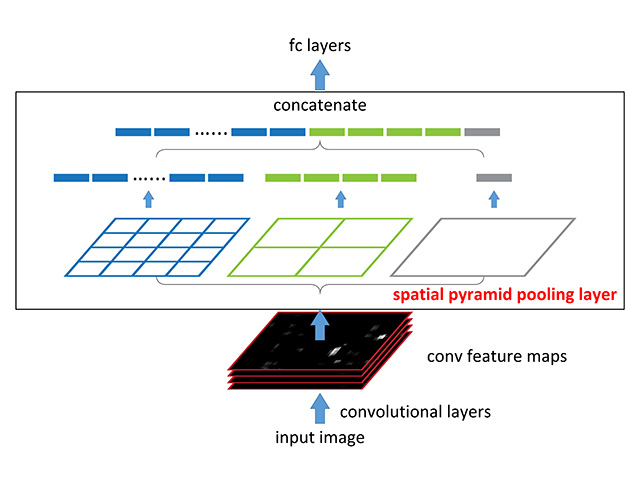
\includegraphics[width=\linewidth]{./img/sppnet.png}
        \caption{Spatial Pyramid Pooling layer. Image taken from:~\cite{sppooling}}\label{fig:sppnet}
    \end{figure}
    
    The pooling operation employed at each level is slightly different from the
    one we have described before. In particular, the one used here is called \textit{Adaptive Pooling}: instead of choosing the window size and the
    stride, we directly choose the output dimensions we want (say $n \times n$). From this, the window and the stride are automatically computed
    as $window = \ceil*{\frac{a}{n}}$ and $stride = \floor*{\frac{a}{n}}$, where $a$ is the dimension of the last conv layer feature maps. As a
    practical example, the VGG16 network~\cite{vgg16} last conv layer feature maps have dimension $512 \times 14 \times 14$\footnote{these are
    the output dimensions when the input image is $224 \times 224$. For bigger (smaller) images, $a$ would be greater (less) than $14$.
    However, using adaptive pooling, the output dimension will be $512 \times 4 \times 4$ regardless of the input size.}.
    If we want an adaptive max pooling of dimension $(4 \times 4)$, the window and the stride are computed as
    $window = \ceil*{\frac{14}{4}} = 4$ and $stride = \floor*{\frac{14}{4}} = 3$. Figure~\ref{fig:sppnet} has a SPP layer with three levels:
    $(4 \times 4) (2 \times 2) (1 \times 1)$. We can easily compute the (fixed) output dimension of this layer. For instance, with the VGG16
    network, the output size is: $(512*4*4) + (512*2*2) + (512*1*1) = 10752$, so we can place a fully-connected layer on top of this SPP and
    we can be sure that the dimension will be the same regardless of the input size.

    \section{Domain-Multiplicative Fusion}
    \subsection{Motivation}
    The architecture of our network, which we called \textbf{Domain-Multiplicative Fusion (DMF)} is inspired from this work~\cite{multfusion}.
    In particular, the authors of~\cite{multfusion} explored two different ways to combine information from multiple sources into the same
    CNN architecture, in the context of action recognition. The first technique, which they called \textit{Feature Amplification},
    consists in an element-wise (hadamard) product between two sources of information: the first was the CNN feature maps and the second
    was the optical flow~\cite{opticalflow} information. The rationale was that through the multiplication, CNN feature maps information
    would detect important features for the action recognition task, and optical flow information would amplify (cancel out) important regions
    in the feature maps with respect to the task of detecting motion.
    Then the author proposed another method to combine different sources, which they called \textit{Multiplicative Fusion}. This method combines
    the feature maps coming from two different CNNs into a merged representation which is then propagated through the fully-connected layers.
    In particular, they employed a layer that performs a linear combination of feature maps (the coefficients of the combination that are learnable
    parameters).

    \begin{figure}[h!]
        \centering{}
        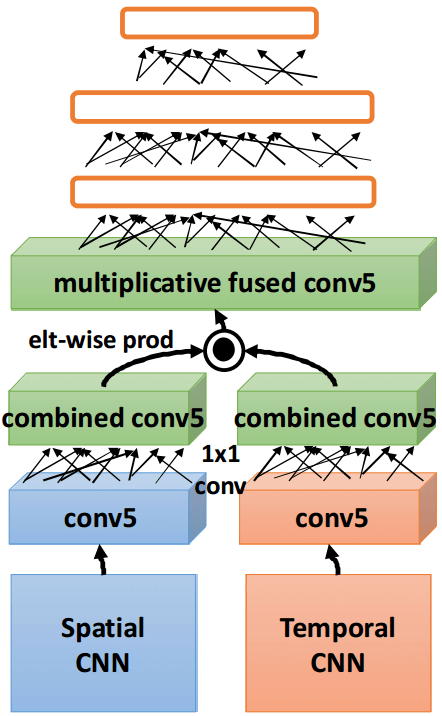
\includegraphics[width=.5\linewidth]{./img/multfusion.png}
        \caption{Multiplicative-Fusion architecture. Image taken from~\cite{multfusion}}\label{fig:multfusion}
    \end{figure}

    \subsection{Architecture Design}
    Although we draw the idea of combining knowledge through multiplication from~\cite{multfusion}, our architecture is quite different from
    theirs, as is the learning task. First of all, let's recap our domain adaptation task and setting. We have two datasets which were drawn
    from two different distributions: the \textit{source} dataset $(X_{s}, Y_{s})$ was drawn from $P_{s}(X, Y)$, and the \textit{target}
    dataset $(X_{t})$ was drawn from $P_{t}(X)$, with $P_{s} \neq P_{t}$. Our learning task is to design a model that learns how to infer
    $Y_{t}$ given $(X_{s}, X_{t}, Y_{s})$. Our method can be summarized in the following way:
    \begin{enumerate}
        \item We train a CNN with a binary classifier on top of it to discriminate between source and target samples. The source samples are
            assigned a label of $0$, and the target samples a label of $1$. The CNN ends with a single sigmoid unit, which outputs the
            probability of the sample being a target sample:
            $$ P(Y = 1 | X) = \hat{y} $$
            This model is trained using the binary-cross-entropy loss function and stochastic gradient descent.
        \item Our modification of the Grad-CAM technique is used to generate activation maps from the previous CNN\@. In particular,
            for each image, we generate a map of the regions that would make the classifier change its decision, from source to target or
            vice-versa. The activations are of the last conv layer, which has a more compact and meaningful representation, as the author
            of Grad-CAM also pointed out.
        \item The maps are integrated into a final CNN that performs object classification. The final architecture can be seen in figure
            (FIG). From the input layer to the last conv layer, the architecture is the same as a standard CNN\@. Then, the output
            feature maps are replicated, 
    \end{enumerate}

    \begin{figure}[h!]
        \centering{}
        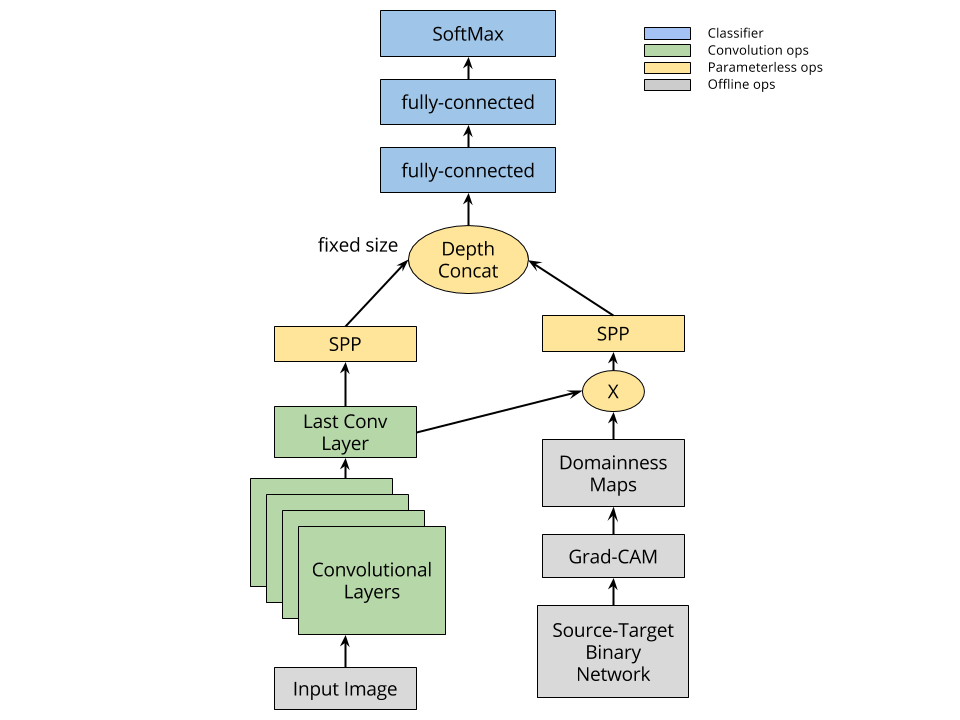
\includegraphics[width=\linewidth]{./img/dmf-architecture.png}
        \caption{Domain-Multiplicative Fusion architecture.}\label{fig:dmf-architecture}
    \end{figure}

    \newline
    We also combine two different networks in our model, but the two are trained separately, with the binary
    network trained first and then used to generate Grad-CAM maps, and the object classification network trained after using the maps.

\end{document}












